\documentclass[french]{beamer}


%%% Style
%%% Gabarit de présentation du DMS
\RequirePackage{graphicx}
\usepackage{colortbl}


%%% Couleurs
\definecolor{bleu-udem}{RGB}{0, 107, 182}
\definecolor{gris-udem}{RGB}{102, 102, 102}
\definecolor{rouge}{RGB}{204, 0, 0}
\definecolor{vert}{RGB}{153, 204, 0}

\usecolortheme{lily}  % désinstalle les couleurs par défaut
\setbeamercolor*{normal text}{fg=black,bg=white}
\setbeamercolor*{alerted text}{fg=rouge}
\setbeamercolor*{example text}{fg=vert}
\setbeamercolor*{structure}{fg=black}

\setbeamercolor*{block title}{fg=white,bg=gris-udem}
\setbeamercolor*{block title alerted}{fg=white,bg=gris-udem}
\setbeamercolor*{block title example}{fg=white,bg=gris-udem}

\setbeamercolor*{block body}{bg=black!10}
\setbeamercolor*{block body alerted}{bg=black!10}
\setbeamercolor*{block body example}{bg=black!10}

\setbeamercolor{item}{fg=bleu-udem}
\setbeamercolor{background canvas}{bg=gris-udem!5}


%%% Liens
\hypersetup{
  colorlinks=true,
  pdfnewwindow=true,
  linkcolor=gris-udem,
  citecolor=bleu-udem,
  filecolor=bleu-udem,
  urlcolor=bleu-udem
}


%%% Canva
\newlength{\textmarginL}
\newlength{\textmarginR}
\setlength{\textmarginL}{7.5mm}
\setlength{\textmarginR}{3.5mm}
\setbeamersize{text margin left=\textmarginL, text margin right=\textmarginR}
\newlength{\titleseparator}
\setlength{\titleseparator}{.71\paperwidth}  % distance entre le côté gauche et la barre horizontale (Page titre)
\newenvironment{changemargin}[2]{%
  \begin{list}{}{%
    \setlength{\topsep}{0pt}%
    \setlength{\leftmargin}{#1}%
    \setlength{\rightmargin}{#2}%
    \setlength{\listparindent}{\parindent}%
    \setlength{\itemindent}{\parindent}%
    \setlength{\parsep}{\parskip}%
  }%
  \item[]}{\end{list}}

%%% Images et logo
\newcommand{\insertslidelogo}{\rule{0pt}{.14\paperheight}} % .14\paperheight = .22\paperwidth
\newcommand{\slidelogo}{
  \renewcommand{\insertslidelogo}{
	
\includegraphics[height=.14\paperheight]{figures/logos/mila}
  }
}
\newcommand{\inserttitlelogo}{\rule{0pt}{.16\paperheight}}  % .16\paperheight = .25\paperwidth
\newcommand{\titlelogo}{
  \renewcommand{\inserttitlelogo}{
	
\includegraphics[height=.16\paperheight]{figures/logos/mila}
  }
}
\newcommand{\inserttitleimage}{\rule{0pt}{.28\paperheight}}
\newcommand{\titleimage}[1]{
  \renewcommand{\inserttitleimage}{
  \includegraphics[height=.28\paperheight, keepaspectratio=true]{#1}
  }
}


%%% Page titre
\setbeamertemplate{title page}{
\begin{changemargin}{-\textmarginL}{-\textmarginR}
\begin{tabular}{@{}r!{\color{bleu-udem}\vline}@{}l@{}}
 & \inserttitlelogo\\
\inserttitleimage & \\
\rule{0pt}{20pt}
\parbox{\titleseparator}{\flushright\Large{\inserttitle}} & \\
\parbox{\titleseparator}{\flushright\small{\insertsubtitle}}  & \\
\rule{0pt}{24pt}
\parbox{\titleseparator}{\flushright\insertauthor} & \\
\parbox{\titleseparator}{\flushright\insertinstitute}  & \\
\rule{0pt}{18pt}
\parbox{\titleseparator}{\flushright\small{\insertdate}} & \\
\end{tabular}
\end{changemargin}
}


%%% Entête
\setbeamertemplate{frametitle}{%
\vskip-33pt\parbox[c]{.68\paperwidth}{\large\insertframetitle}\vskip4pt%
}
\setbeamertemplate{headline}{%
\hfill\insertslidelogo

\color{bleu-udem}\rule{.98\paperwidth}{.07pt}%
}


%%% Pied de page
\beamertemplatenavigationsymbolsempty
\newcommand{\numsubsectionname}{}
\newcommand{\showsubsection}{
  \renewcommand{\numsubsectionname}{%
	\thesection.\thesubsection \; \insertsubsection
  }
}
\newcommand{\insertfootlinetext}{}
\newcommand{\footlinetext}[1]{
  \renewcommand{\insertfootlinetext}{#1}
}
\setbeamertemplate{footline}{
{\hfill\color{bleu-udem}\rule{.98\paperwidth}{0.07pt}}%
\vskip4pt%
\color{gris-udem}%
\rule{0.02\paperwidth}{0pt}%
\numsubsectionname
\hfill%
\mbox{\insertfootlinetext\qquad\qquad\insertframenumber}%
\rule{\textmarginR}{0pt}%
\vskip4pt%
}



%%% Extensions utiles pour le français
\usepackage[french]{babel}
\usepackage[utf8]{inputenc}
\usepackage[T1]{fontenc}

\usepackage{xcolor}

%%% Extensions utiles pour les math
\usepackage{amsmath}
\usepackage{amsfonts}
\usepackage{bbold}
\usepackage{mathtools}

\DeclareMathOperator*{\argmin}{arg\,min}

%%% Extensions pour les figures
\usepackage{graphicx}
\usepackage{subfig}
\usepackage{tikz}

%%% Bibliographie
\usepackage{bibentry}

%%% Informations sur la présentation
\author{Patrice Béchard}
\institute[DIRO]{\small{Département d'informatique et de recherche opérationnelle}}
\title{Apprentissage profond}
\subtitle{Introduction et applications en physique}
\date{\today}


%%% Préférences (Propre au thème du DMS)
\slidelogo
\titlelogo
\titleimage{figures/deep_learning_v2.png}  % Image à afficher sur la page titre
\footlinetext{  % À utiliser surtout pour les congrès
\insertshorttitle\quad\insertshortdate\quad\insertshortinstitute
}


\def\signed #1{{\leavevmode\unskip\nobreak\hfil\penalty50\hskip2em
  \hbox{}\nobreak\hfil(#1)%
  \parfillskip=0pt \finalhyphendemerits=0 \endgraf}}

\newsavebox\mybox
\newenvironment{aquote}[1]
  {\savebox\mybox{#1}\begin{quote}}
  {\signed{\usebox\mybox}\end{quote}}

\usepackage{ragged2e}


%%% Début
\begin{document}


\begin{frame}[plain, t]
  \titlepage
\end{frame}


\begin{frame}{Plan de l'exposé}
  \tableofcontents
\end{frame}


%\showsubsection  % À utiliser surtout pour les cours

\section{L'IA dans la culture populaire}
\subsection*{L'IA dans la culture populaire}

\begin{frame}{L'IA dans la culture populaire}
\begin{center}
\begin{tikzpicture}
  \node (img1) {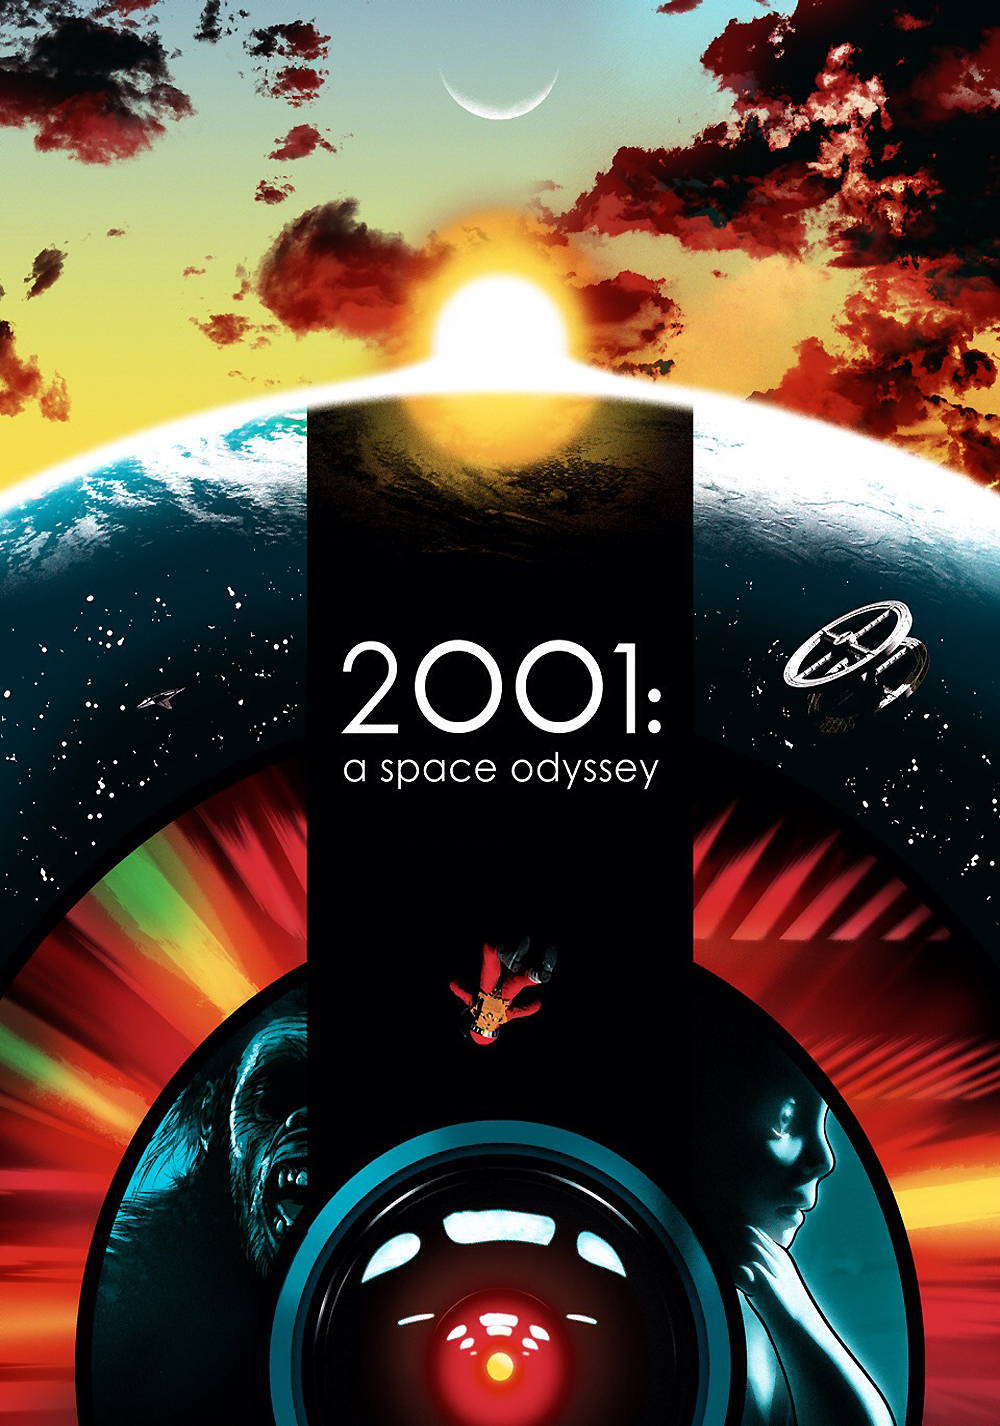
\includegraphics[height=3cm]{figures/movies/2001_space_odyssey}};
  \pause
  \node (img2) at (img1.south east) {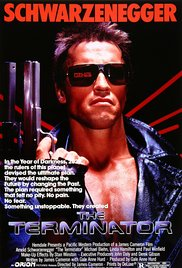
\includegraphics[height=3cm]{figures/movies/terminator}};
  \pause
  \node (img3) at (img2.north east) [yshift=1cm] {
\includegraphics[height=3cm]{figures/movies/tron}};
  \pause
  \node (img4) at (img1.south west) [yshift=0.5cm]{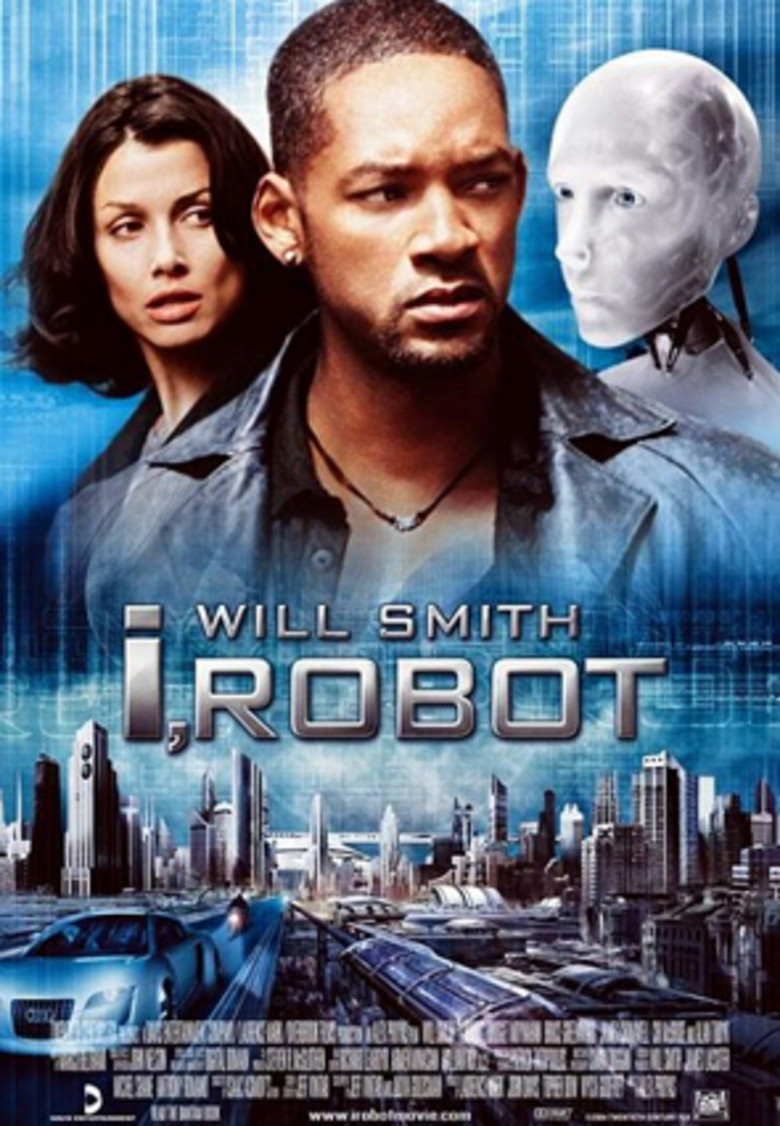
\includegraphics[height=3cm]{figures/movies/i_robot}};
  \pause
  \node (img5) at (img4.north west) [yshift=0.5cm]{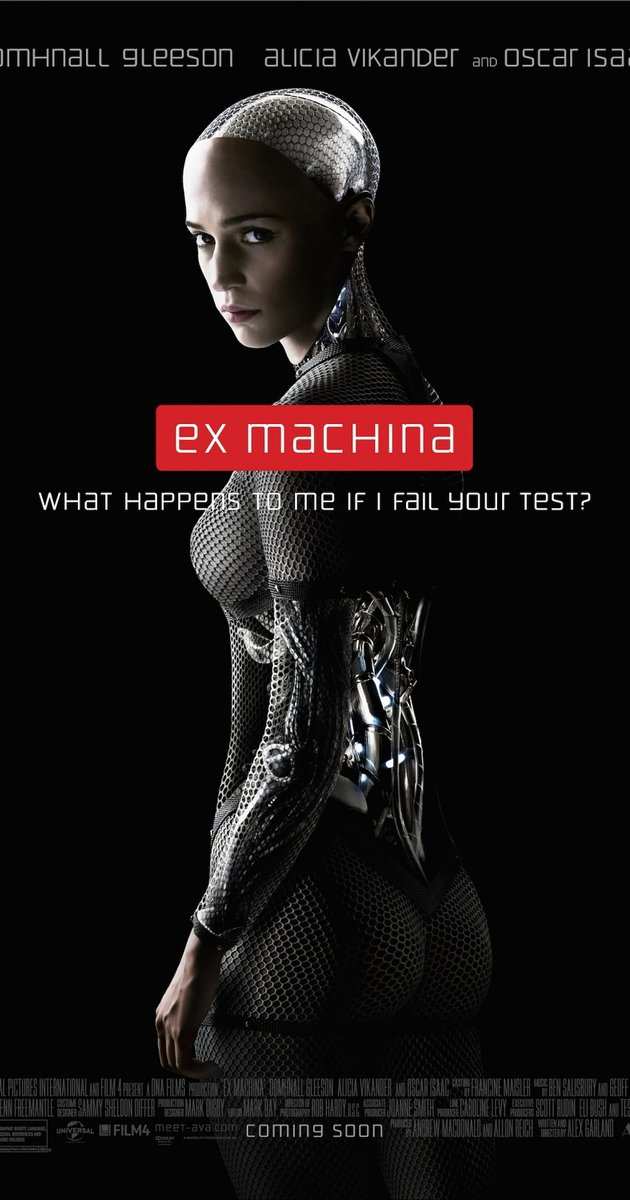
\includegraphics[height=3cm]{figures/movies/ex_machina}};
  \pause
  \node (img6) at (img2.south east) [yshift=0.5cm]{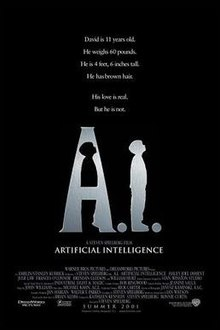
\includegraphics[height=3cm]{figures/movies/artificial_intelligence}};
  \pause
  \node (img7) at (img4.south east) [yshift=-0.5cm]{
\includegraphics[height=3cm]{figures/movies/wall_e}};
  \pause
  \node (img7) at (img4.south west) [yshift=0.5cm]{
\includegraphics[height=3cm]{figures/movies/mega_man}};
  \pause
  \node (img8) at (img3.south east) [yshift=0.5cm, xshift=0.5cm]{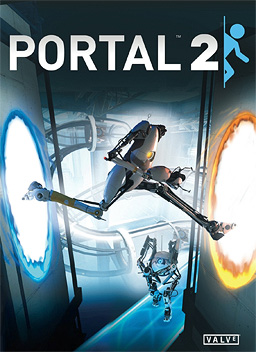
\includegraphics[height=3cm]{figures/movies/portal}};
  \pause
  \node (img9) at (img8.south east) [yshift=-0.5cm, xshift=-0.5cm]{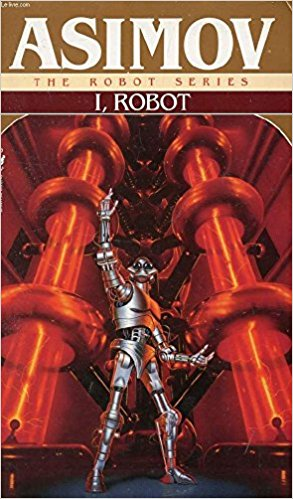
\includegraphics[height=3cm]{figures/movies/i_robot_asimov}};
\end{tikzpicture}
\end{center}
\end{frame}

\section{Histoire de l'IA et de l'apprentissage automatique}

\begin{frame}{Histoire de l'IA et de l'apprentissage automatique}
\begin{description}

	\item[Antiquité] Idée des robots conscients / automates (Égypte, Grèce)
	\item[17\textsuperscript{e} siècle] Descartes, Hobbes et la philosophie mécaniste. \\ Leibniz et la Caractéristique universelle.
	\item[20\textsuperscript{e} siècle] Boole, Russell et les fondements de la logique. \\ Hilbert : Peut-on formaliser tout raisonnement mathématique? \\
										Réponses de Gödel, Turing, Church...
\end{description}
\textbf{Conclusions :}
\begin{itemize}
	\item Il existe des limites à ce que l'on peut accomplir avec la logique.
	\item Dans ces limites, toute forme de raisonnement mathématique peut être mécanisé.
\end{itemize}
\end{frame}

\begin{frame}{Histoire de l'IA et de l'apprentissage automatique}
\vspace{1cm}
\begin{changemargin}{-1cm}{-1cm} 
\begin{description}	
	\item [1943] Pitts \& McCulloch proposent l'idée du neurone artificiel \cite{mcculloch1943logical}
	\item [1950] Test de Turing \cite{turing1950computing}
	\item [1957] Rosenblatt propose l'algorithme du perceptron \cite{rosenblatt1958perceptron}
\end{description}
\vspace{1cm}
\begin{center}
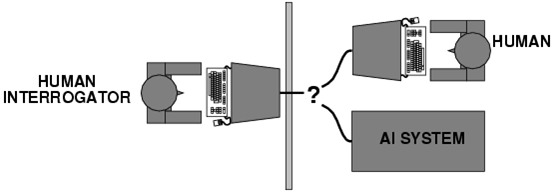
\includegraphics[height=3cm]{figures/turing_test}
\end{center}
\end{changemargin} 
\end{frame}

\begin{frame}{Histoire de l'IA et de l'apprentissage automatique}
\begin{description}
	\item [1960 - 2000] Hauts et bas dans le milieu.
\end{description}
\vspace{1cm}
\textbf{Problèmes}
\begin{itemize}
	\item Puissance des ordinateurs toujours limitée
	\item Données souvent insuffisantes
	\item Paradoxe de Moravec
\end{itemize}
\end{frame}


\begin{frame}{Histoire de l'IA et de l'apprentissage automatique}
\textbf{Paradoxe de Moravec}

\justify
\begin{aquote}{Hans Moravec\cite{moravec1988mind}}
"It is comparatively easy to make computers exhibit adult-level performance in solving problems on intelligence tests or playing checkers, and difficult or impossible to give them the skills of a one-year-old when it comes to perception and mobility."
\end{aquote}

\end{frame}

\begin{frame}{Histoire de l'IA et de l'apprentissage automatique}
\textbf{Avancées récentes}
\begin{description}
 \item [1998] Deep Blue bat Garry Kasparov aux échecs.
 \item [2011] Watson bat les deux plus grands champions à \textit{Jeopardy!}
 \item [2016] AlphaGo bat Lee Sedol au jeu de Go.
 \item [2017] AlphaZero atteint un niveau surhumain aux jeux de Go, shogi et échecs sans données externes en 24h\cite{silver2017mastering}.
\end{description}
\centering
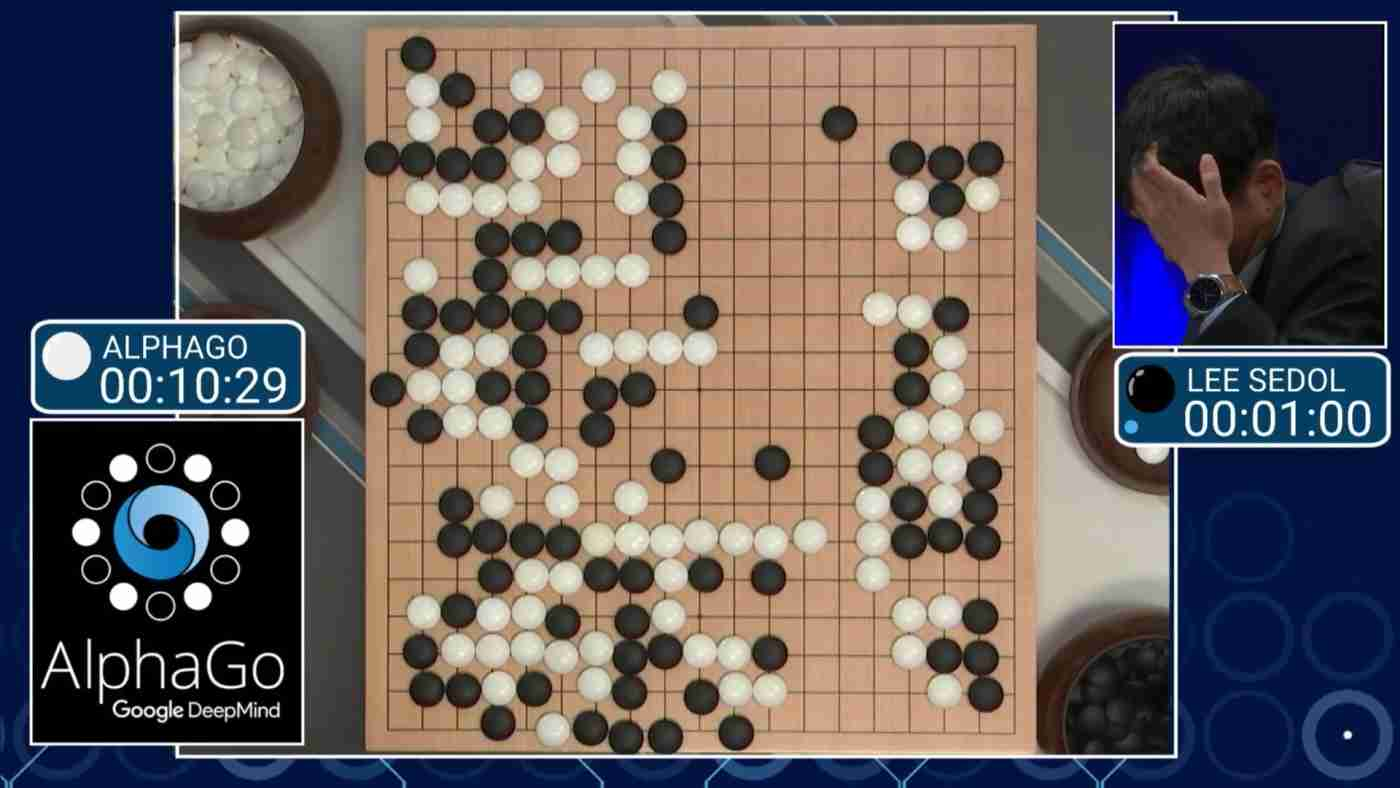
\includegraphics[height=3cm]{figures/alphago}
\end{frame}

\begin{frame}{Histoire de l'IA et de l'apprentissage automatique}
\textbf{Autres domaines où les progrès sont fulgurants}
\begin{itemize}
 \item Vision par ordinateur
 \item Reconnaissance de la parole
 \item Traduction automatique
 \item Génération d'images
 \item et beaucoup plus...
\end{itemize}

\end{frame}

\section{Bases de l'apprentissage automatique}

\begin{frame}{Bases de l'apprentissage automatique}
\textbf{Deux approches à l'intelligence artificielle}
\vspace{0.5cm}

\begin{columns}[T] % align columns
\begin{column}{.48\textwidth}
\begin{center}
\underline{IA «classique» symbolique}
\end{center}
\begin{itemize}
	\item Fondé sur le \\raisonnement logique
	\item Règles codées à la main \\(\texttt{if... else...})
	\item Pas de gestion de l'incertain
\end{itemize}

\end{column}%
\hfill%
\begin{column}{.48\textwidth}
\begin{center}
\underline{Apprentissage automatique}
\end{center}
\begin{itemize}
	\item Apprendre les paramètres à partir d'exemples
	\item Approche probabiliste
	\item Objectif : \textbf{généralisation}
\end{itemize}
\end{column}%
\end{columns}
\end{frame}

\begin{frame}{Bases de l'apprentissage automatique}
\textbf{Types de problèmes}
\vspace{0.5cm}

\begin{itemize}
	\item Apprentissage supervisé
	\begin{itemize}
		\item Régression
		\item Classification
	\end{itemize}
	\item Apprentissage non-supervisé
	\begin{itemize}
		\item Réduction de dimensionalité, clustering, détection d'anomalie, ...
	\end{itemize}
	\item Apprentissage par renforcement
\end{itemize}
\end{frame}

\begin{frame}{Bases de l'apprentissage automatique}
\textbf{Apprentissage supervisé}
\vspace{0.5cm}
\begin{itemize}
	\item Ensemble de données $\mathcal{D_{\mathrm{train}}} = \{(x^{(1)}, y^{(1)}), (x^{(2)}, y^{(2)}), \dots,  (x^{(N)}, y^{(N)})\}$.
	\item Le modèle prédit une sortie $f(x^{(i)})$ en fonction de l'entrée $x^{(i)}$. On veut que le modèle prédise la cible $y^{(i)}$.
	\item Lors de la phase d'entraînement, le modèle ajuste ses paramètres $\Theta$ dans le but de minimiser le risque empirique $\hat{R}$ selon une fonction de coût $\mathcal{L}(y, f(x))$
\end{itemize}
$$
\hat{R} = \frac{1}{N} \sum_{i=1}^N \mathcal{L}\left(y^{(i)}, f(x^{(i)})\right)
\qquad
\Theta^* = \argmin_\Theta \hat{R}(f, \mathcal{D}_{train})
$$
\end{frame}

\begin{frame}{Bases de l'apprentissage automatique}
\textbf{Quelques fonctions de coût...}
\vspace{.5cm}
\begin{itemize}
	\item Erreur quadratique (régression) : 
	\vspace{-.2cm}
	$$ \mathcal{L}(y, f(x)) = ||y-f(x)||_2^2$$
	\item Erreur de classification : 
	\vspace{-.2cm}
	$$\mathcal{L}(y, f(x)) = \mathbb{1}_{\{y \neq f(x) \}}$$
	\item Entropie croisée binaire : 
	\vspace{-.2cm}	
	$$ \mathcal{L}(y, f(x)) = -y \log f(x) + (1-y) \log (1-f(x))$$
	\item Moins log-vraisemblance : 
	\vspace{-.2cm}	
	$$ \mathcal{L}(y, f(x)) = - \log f(x)_y $$
\end{itemize}
\end{frame}

\begin{frame}{Bases de l'apprentissage automatique}
\textbf{Estimer l'erreur de généralisation}
\vspace{.5cm}
\begin{itemize}
	\item But de l'apprentissage machine : \textbf{généralisation}
	\item On test le modèle entraîné sur des exemples jamais vus auparavant :
	\vspace{-.2cm}
	$$\mathcal{D}_{\mathrm{test}} = \{ (x^{(1')}, y^{(1')}), (x^{(2')}, y^{(2')}), \dots, (x^{(N')}, y^{(N')}) \}$$
\end{itemize}
\begin{center}
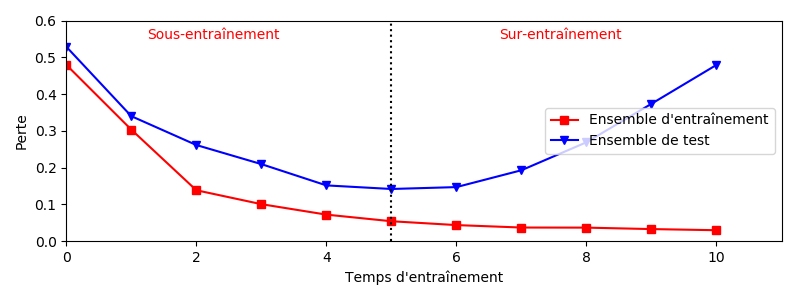
\includegraphics[height=3.5cm]{figures/learning_curve}
\end{center}
\end{frame}

\begin{frame}{Bases de l'apprentissage automatique}
\textbf{Exemple : Prédiction du prix des maisons à Boston \cite{harrison1978hedonic}}
\vspace{0.5cm}
\begin{columns}[T] % align columns
\begin{column}{.48\textwidth}
\begin{itemize}
	\item Problème de régression
	\item \textbf{Entrée} : 13 traits caractéristiques ($\in \mathbb{R}^{13}$)\\ ex: Nb. de chambres, Taux de criminalité, ...
	\item \textbf{Sortie} : Prix de la maison ($\in \mathbb{R}$)
\end{itemize}
\end{column}%
\hfill%
\begin{column}{.48\textwidth}
\centering
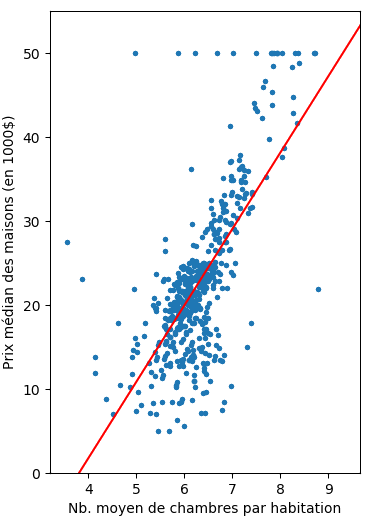
\includegraphics[height=6cm]{figures/boston}
\end{column}%
\end{columns}
\end{frame}

\begin{frame}{Bases de l'apprentissage automatique}
\vspace{0.5cm}
\textbf{Exemple : Classification de chiffres manuscrits \cite{lecun1998mnist}}
\begin{itemize}
	\item Problème de classification
	\item Entrée : Image 28x28 px
	\item Sortie : Chiffre de 0 à 9
\end{itemize}
\vspace{0.5cm}
\begin{center}
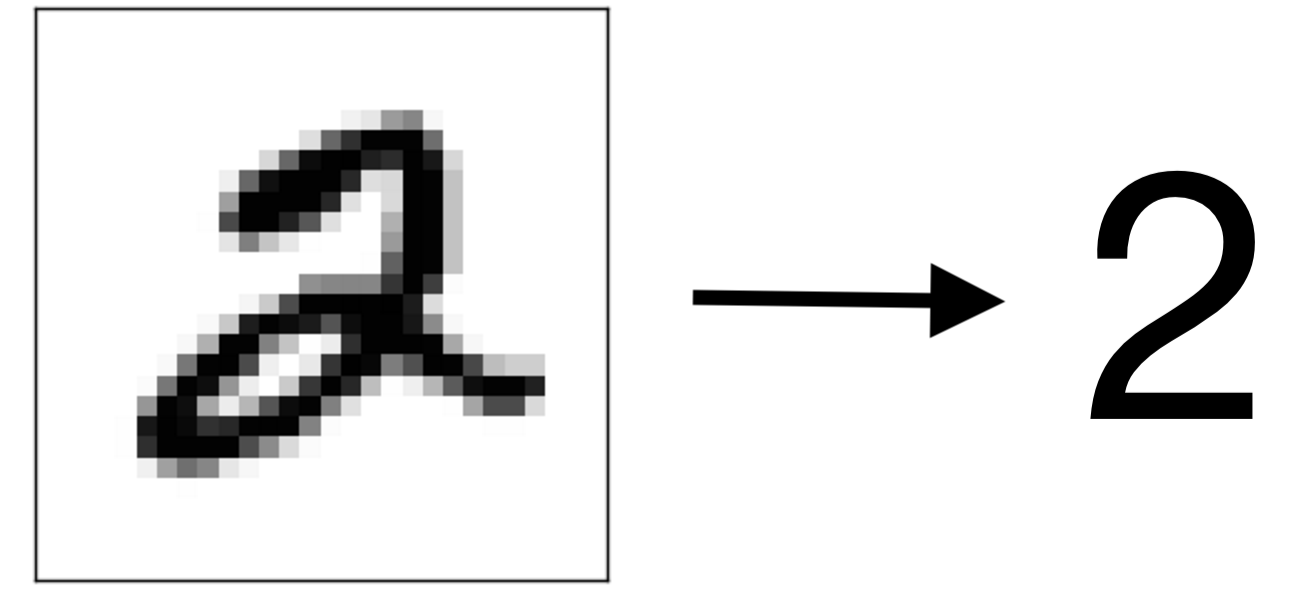
\includegraphics[height=3cm]{figures/mnist-2}
\end{center}
\end{frame}

\section{Réseaux de neurones et apprentissage profond}

\subsection{Principes et fondements}

\begin{frame}{Réseaux de neurones et apprentissage profond}
\begin{columns}[T]
\begin{column}{.48\textwidth}
\begin{center}
\underline{Neurone biologique}\\
\vspace{.5cm}
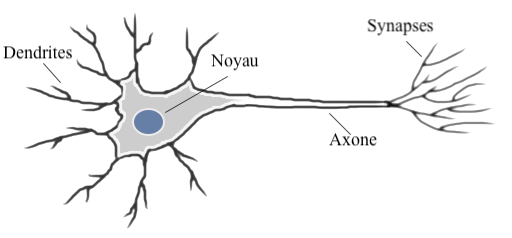
\includegraphics[width=\linewidth]{figures/biological_neuron}
\end{center}
\end{column}
\hfill
\begin{column}{.48\textwidth}
\begin{center}
\underline{Neurone artificiel}\\
\vspace{.5cm}
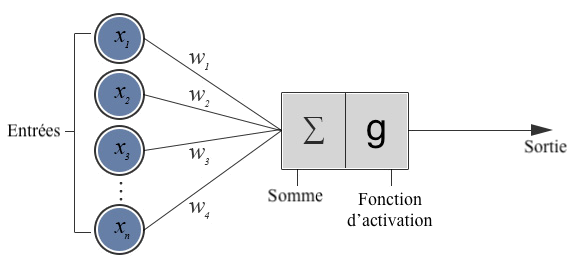
\includegraphics[width=\linewidth]{figures/artificial_neuron}
\end{center}
\end{column}
\end{columns}
\end{frame}

\begin{frame}{Réseaux de neurones et apprentissage profond}
\textbf{Quelques fonctions d'activation}
\vspace{-.5cm}
\begin{columns}[T]
\begin{column}{.48\textwidth}
\begin{center}
\underline{Linéaire} : $g(x) = x$\\
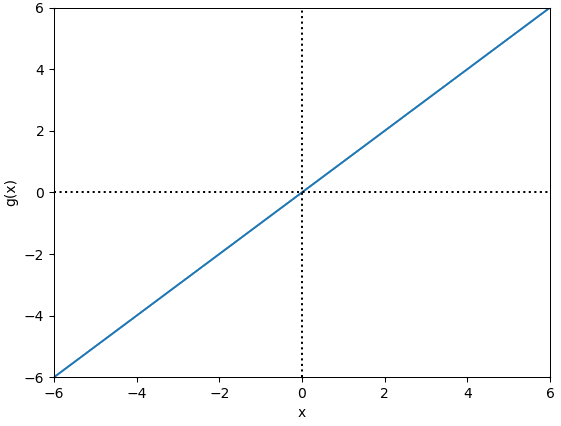
\includegraphics[width=.6\linewidth]{figures/linear}\\
\underline{ReLU} : $g(x) = max(0, x)$\\
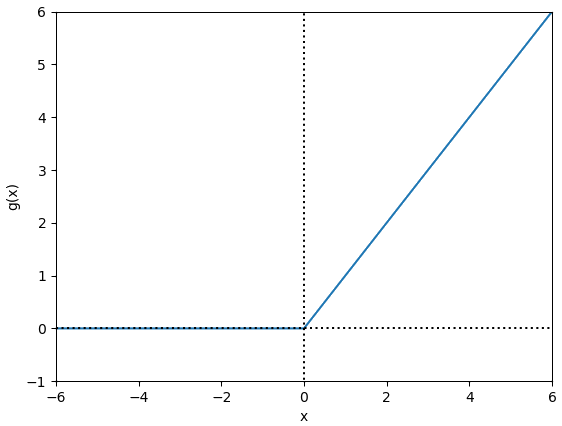
\includegraphics[width=.6\linewidth]{figures/relu}\\
\end{center}
\end{column}
\hfill
\begin{column}{.48\textwidth}
\begin{center}
\underline{Sigmoïde} : $g(x) = \frac{1}{1 + \exp (-x)}$\\
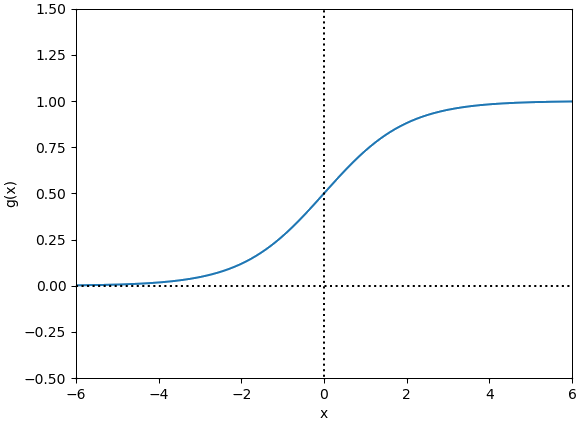
\includegraphics[width=.6\linewidth]{figures/sigmoid}\\
\underline{Tanh} : $g(x) = \tanh(x)$\\
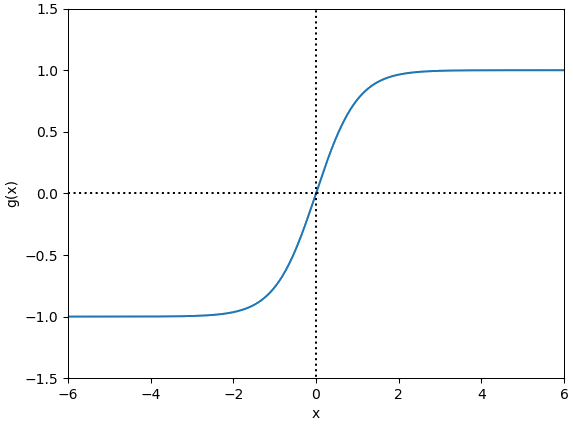
\includegraphics[width=.6\linewidth]{figures/tanh}
\end{center}
\end{column}
\end{columns}
\end{frame}

\begin{frame}{Réseaux de neurones et apprentissage profond}
\textbf{Modèle linéaire : Régression linéaire}
\vspace{0.5cm}
\begin{itemize}
	\item Modèle pour la régression
\end{itemize}
$$ f(\mathrm{x}) = \mathrm{w}^T\mathrm{x} + b = \sum_i \mathrm{w}_i \mathrm{x}_i + b $$
Représentation neuronale :\\
\centering
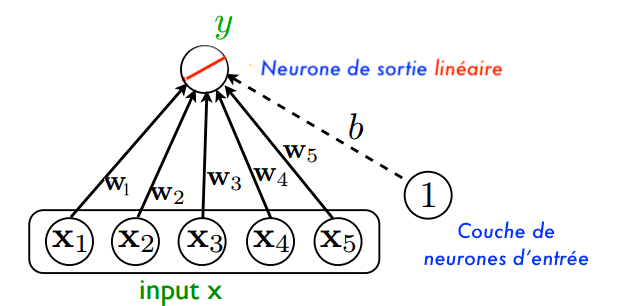
\includegraphics[height=3cm]{figures/linear_regression}
\end{frame}

\begin{frame}{Réseaux de neurones et apprentissage profond}
\textbf{Modèle linéaire : «Régression» logistique}
\vspace{0.5cm}
\begin{itemize}
	\item Modèle pour la classification binaire
\end{itemize}
$$ f(\mathrm{x}) = \mathrm{sigm}\left( \mathrm{w}^T\mathrm{x} + b \right) = \mathrm{sigm}\left( \sum_i \mathrm{w}_i \mathrm{x}_i + b \right) $$
Représentation neuronale :\\
\centering
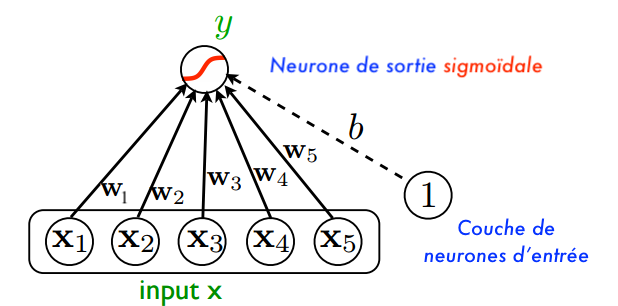
\includegraphics[height=3cm]{figures/logistic_regression}
\end{frame}

\begin{frame}{Réseaux de neurones et apprentissage profond}
\textbf{Problème : ensembles de données non linéairement séparables}
\vspace{-.5cm}
\begin{columns}[T]
\hfill
\begin{column}{.3\textwidth}
\begin{center}
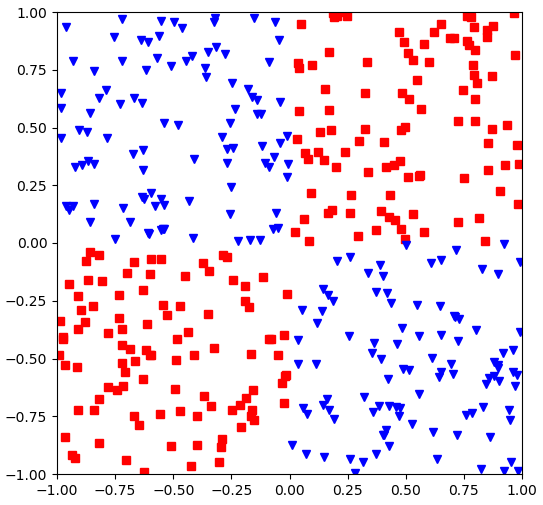
\includegraphics[width=\linewidth]{figures/xor} \\
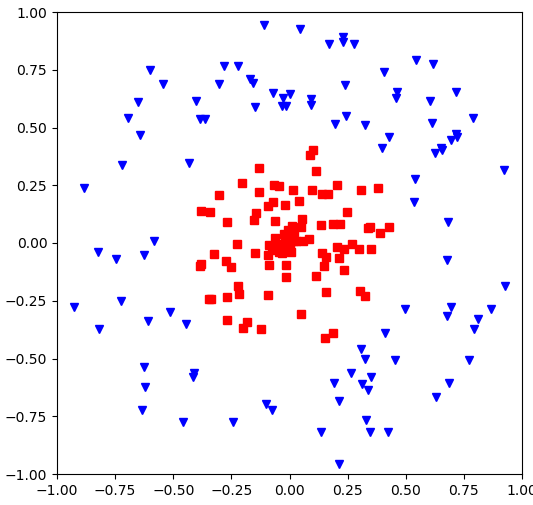
\includegraphics[width=\linewidth]{figures/circle}
\end{center}
\end{column}
\pause
\begin{column}{.3\textwidth}
\vspace{1.5cm}
$$\xrightarrow[\text{deux composantes}]{\text{Multiplier les}}$$
\vspace{2cm}
$$ \xrightarrow[\text{polaires}]{\text{Coordonnées}} $$
\end{column}
\begin{column}{.3\textwidth}
\begin{center}
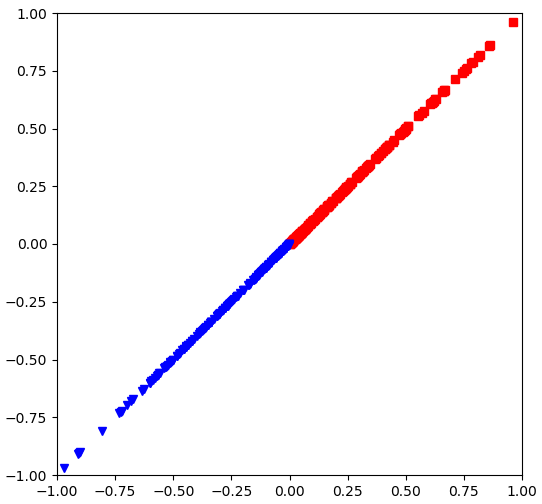
\includegraphics[width=\linewidth]{figures/xor_transform} \\
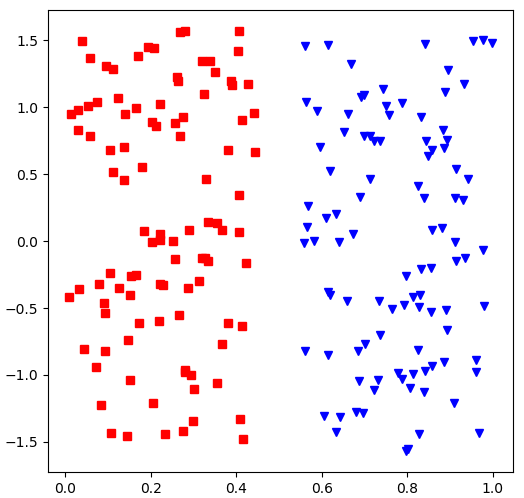
\includegraphics[width=\linewidth]{figures/circle_transform} \\
\end{center}
\end{column}
\hfill
\end{columns}
\end{frame}


\begin{frame}{Réseaux de neurones et apprentissage profond}
\begin{center}
{\Large Comment définir ces nouvelles représentations pour chaque ensemble de données?} \\
\pause
\vspace{1cm}
{\Large{\textcolor{red}{On laisse le modèle les apprendre!}}}
\end{center}
\end{frame}

\begin{frame}{Réseaux de neurones et apprentissage profond}
\textbf{Introduction d'une couche de neurones cachés}

\begin{columns}[T]
\begin{column}{.48\textwidth}
\begin{itemize}
	\item Entrée : $\mathrm{x} \in \mathbb{R}^d$
	\item Paramètres : \\ $W^{(1)} \in \mathbb{R}^{d\times d_h}$, $b^{(1)} \in \mathbb{R}^{d_h}$ \\ $W^{(2)} \in \mathbb{R}^{d_h \times d_o}$, $b^{(2)} \in \mathbb{R}^{d_o}$
	\item Propagation : \\ {\small $h^{(1)}\left(\mathrm{x}) = g^{(1)}(W^{(1), T}\mathrm{x} + b^{(1)}\right)$} \\ {\small$f(\mathrm{x})~=~g^{(2)}\left(W^{(2), T} h^{(1)}(\mathrm{x})~+~b^{(2)}\right)$}
\end{itemize}
\end{column}
\hfill
\begin{column}{.48\textwidth}
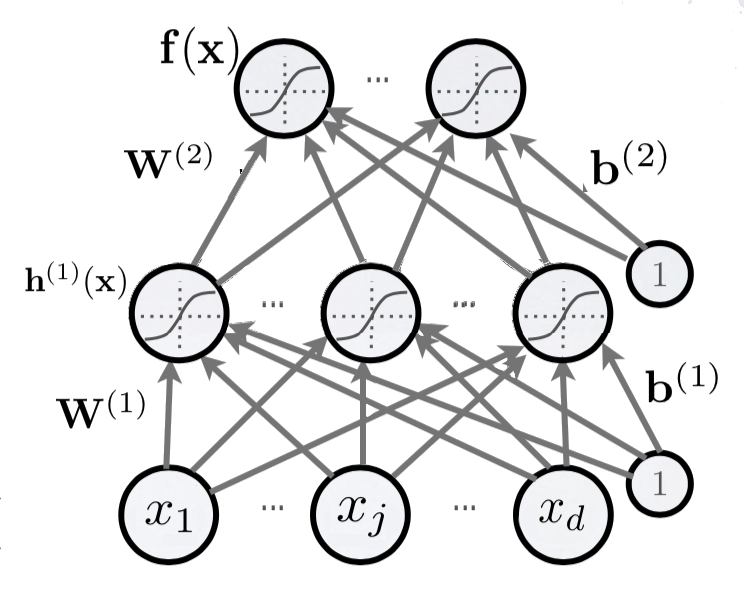
\includegraphics[width=\textwidth]{figures/nn}
\end{column}
\end{columns}
\end{frame}

\begin{frame}{Réseaux de neurones et apprentissage profond}
\textbf{On peut aussi avoir plus d'une couche cachée!}
\begin{columns}[T]
\begin{column}{.48\textwidth}
\begin{itemize}
	\item C'est ce qu'on appelle l'\textbf{apprentissage profond}.
	\item Le nombre de couches cachées ainsi que le nombre de neurones dans chaque couche cachée sont des \textbf{hyperparamètres} que l'utilisateur doit ajuster manuellement.
\end{itemize}
\end{column}
\hfill
\begin{column}{.48\textwidth}
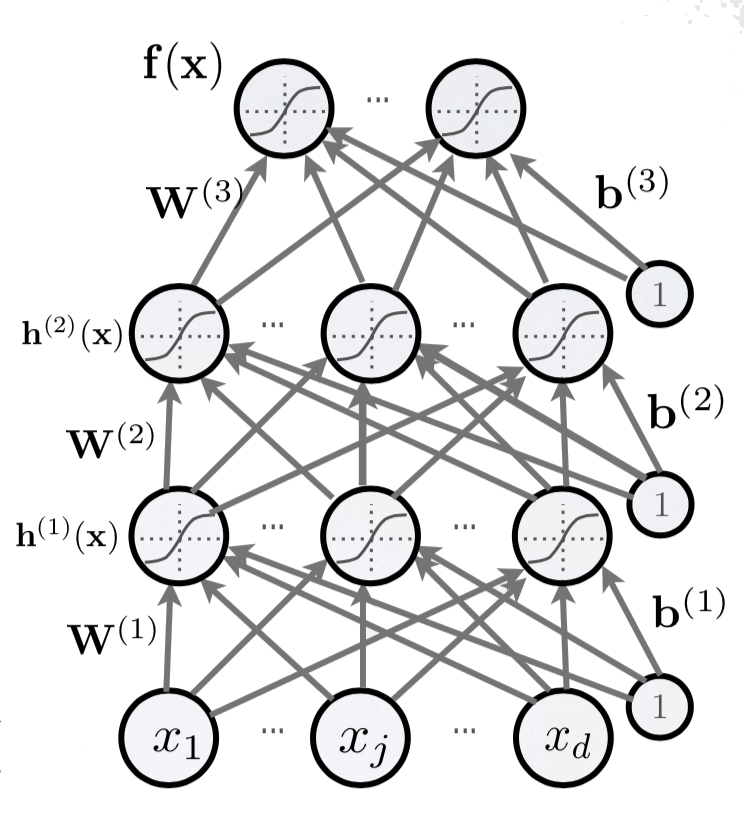
\includegraphics[width=\textwidth]{figures/deep_nn}
\end{column}
\end{columns}
\end{frame}

\begin{frame}{Réseaux de neurones et apprentissage profond}
\textbf{Apprentissage des paramètres : algorithme de rétropropagation}
\begin{columns}[T]
\begin{column}{.52\textwidth}
{\small
\begin{itemize}
	\item On calcule le gradient de la fonction de coût $\nabla \mathcal{L}(f(x), y)$ pour chaque élément du réseau en utilisant la règle de dérivée en chaîne.
	\item On ajuste les paramètres dans la direction opposée du gradient : \\ $$ \theta^{(t+1)} \leftarrow \theta^{(t)} - \eta \nabla_{\theta}\mathcal{L}(f(x), y)^{(t)} $$
	\item Le \textbf{taux d'apprentissage} $\eta$ est un hyperparamètre à déterminer.
	\item On répète pour chaque exemple jusqu'à convergence.
\end{itemize}
}
\end{column}
\hfill
\begin{column}{.52\textwidth}
\only<1>{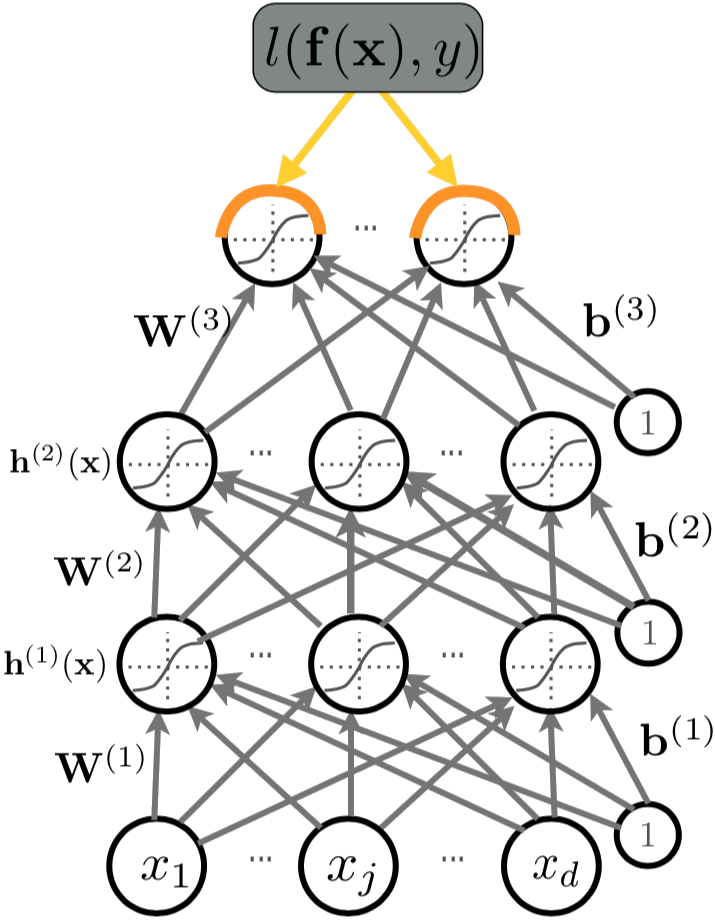
\includegraphics[width=.8\textwidth]{figures/backprop/1}}
\only<2>{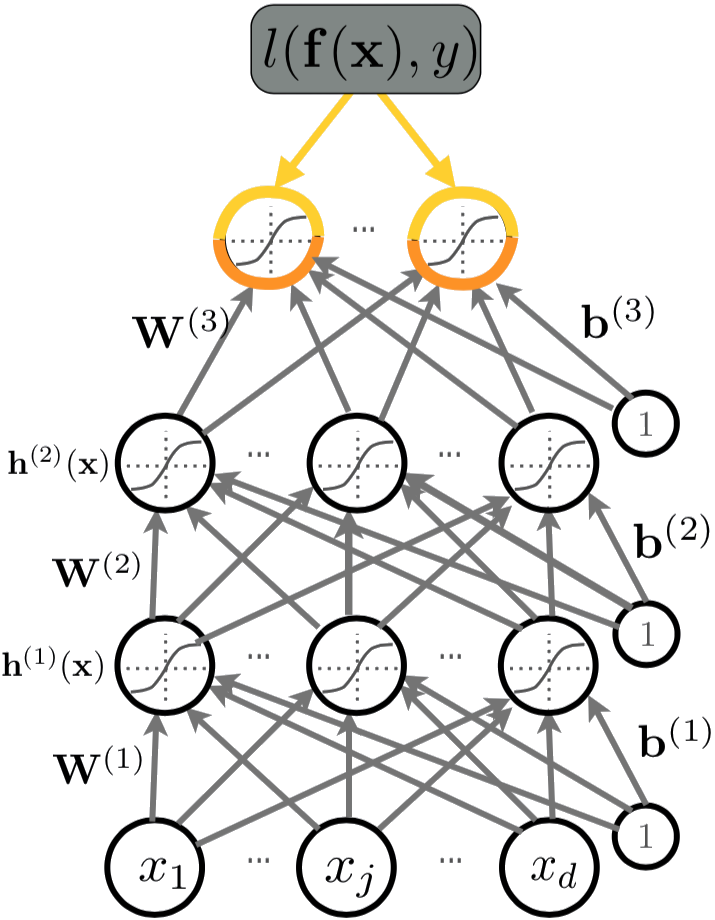
\includegraphics[width=.8\textwidth]{figures/backprop/2}}
\only<3>{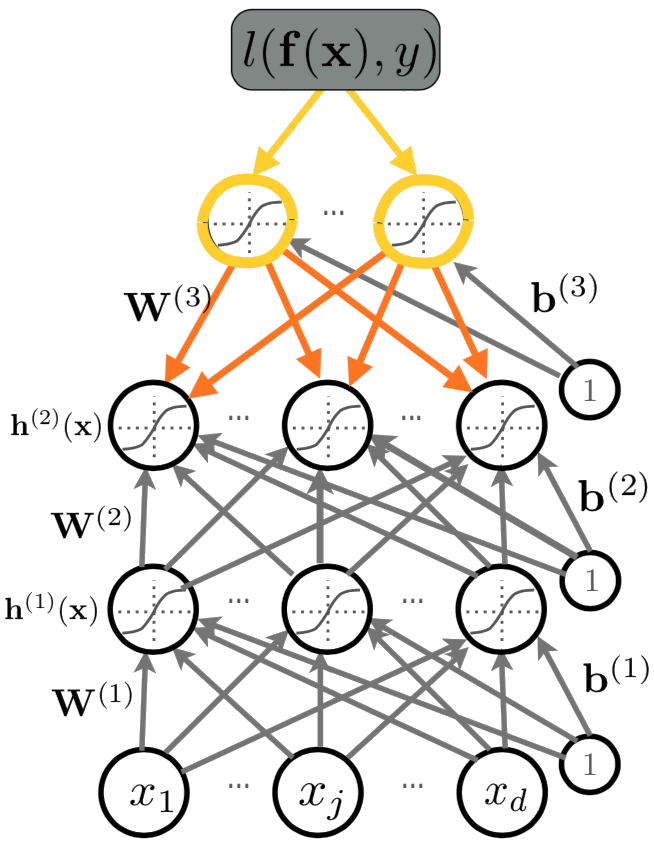
\includegraphics[width=.8\textwidth]{figures/backprop/3}}
\only<4>{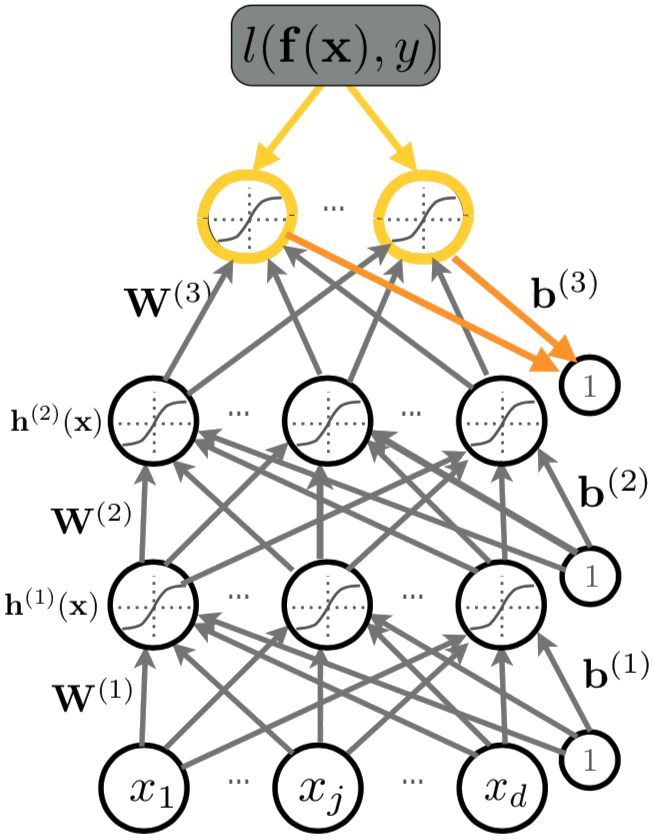
\includegraphics[width=.8\textwidth]{figures/backprop/4}}
\only<5>{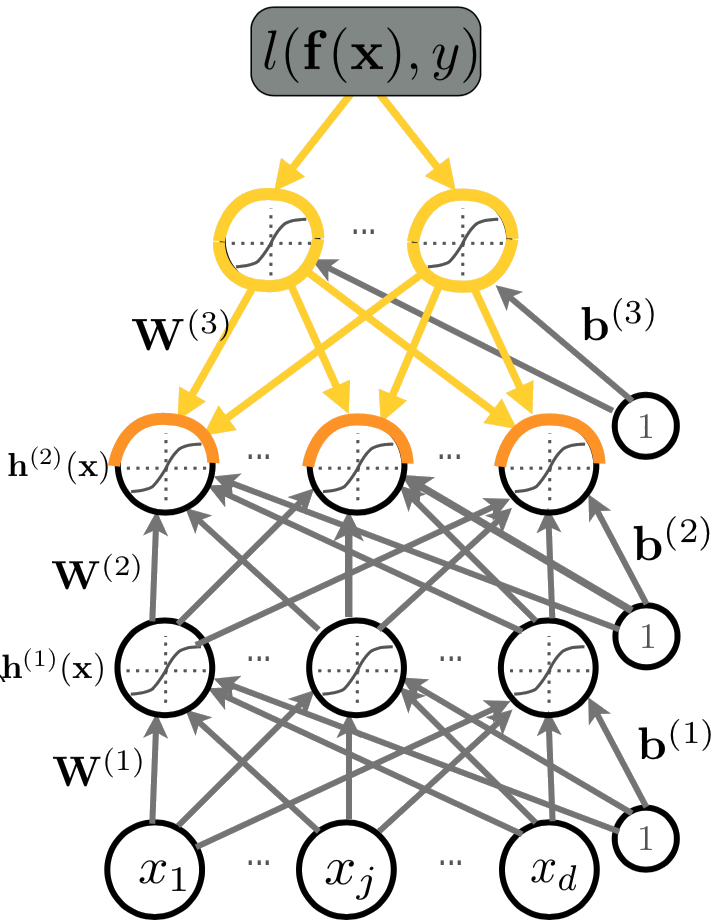
\includegraphics[width=.8\textwidth]{figures/backprop/5}}
\only<6>{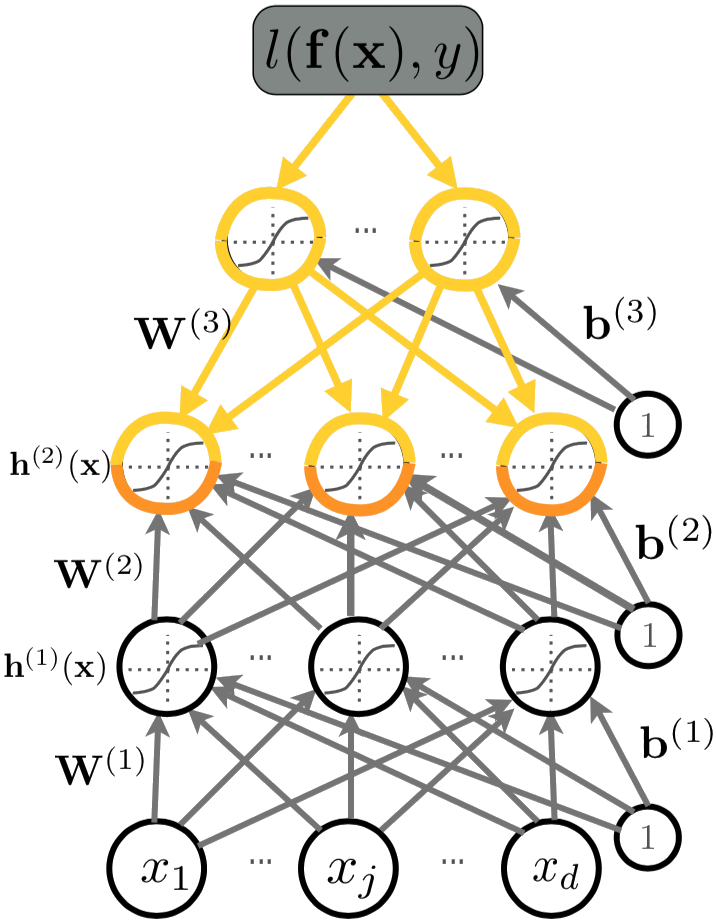
\includegraphics[width=.8\textwidth]{figures/backprop/6}}
\end{column}
\end{columns}
\end{frame}

\begin{frame}{Réseaux de neurones et apprentissage profond}
\begin{center}
Beaucoup d'autres types de réseaux de neurones existent!
\end{center}
\begin{columns}[T]
\begin{column}{.52\textwidth}
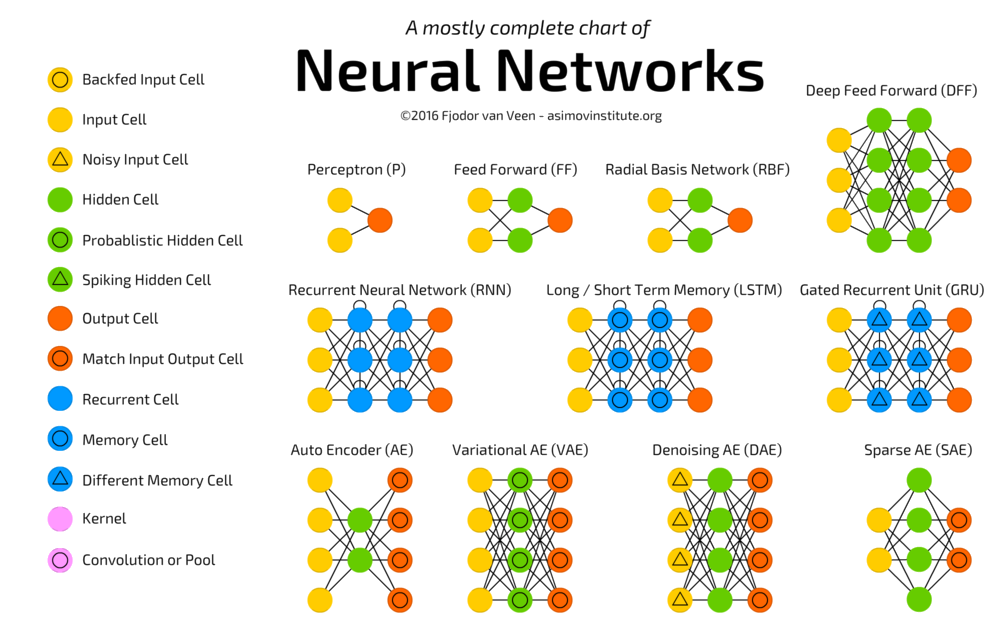
\includegraphics[width=\textwidth]{figures/map_nn_1}
\end{column}
\hfill
\begin{column}{.52\textwidth}
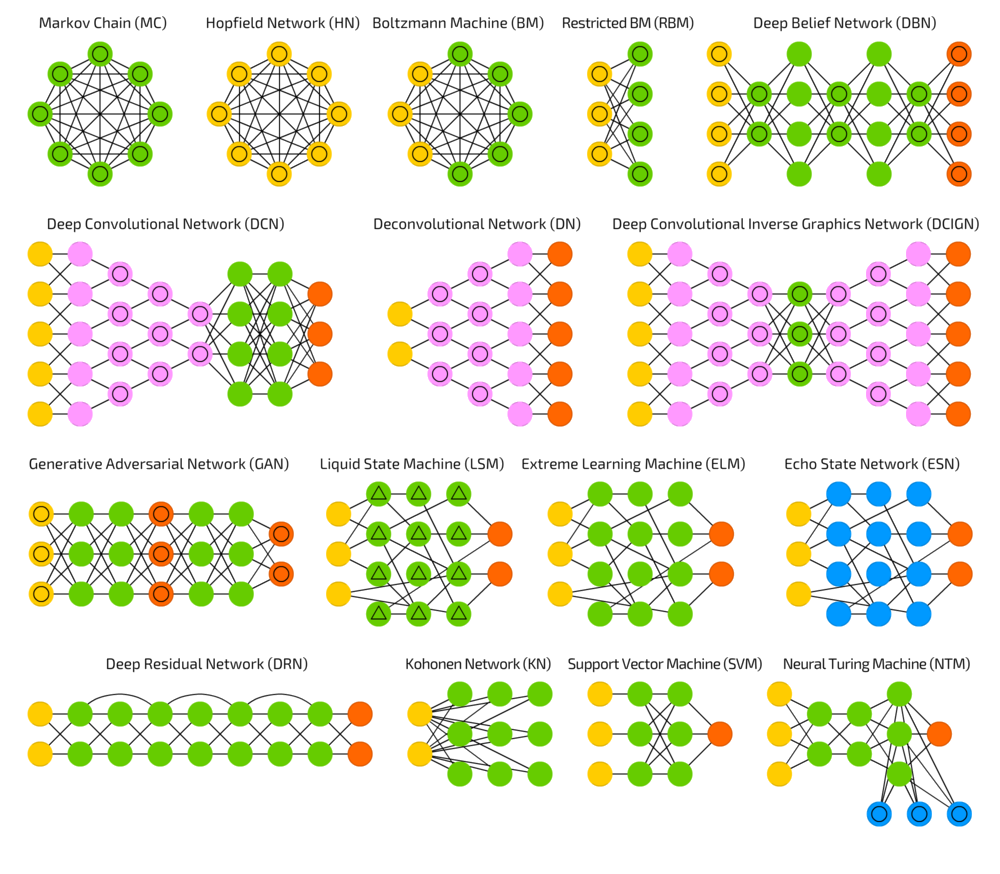
\includegraphics[width=\textwidth]{figures/map_nn_2}
\end{column}
\end{columns}
\end{frame}

\begin{frame}{Réseaux de neurones et apprentissage profond}
\textbf{Réseaux de neurones convolutifs (CNN)}
\begin{itemize}
	\item Grandement utilisé pour la vision par ordinateur
	\item Prend en compte de la connectivité locale des paramètres
	\item Permet d'introduire une invariance dans la compréhension des paramètres
	
\end{itemize}
\begin{center}
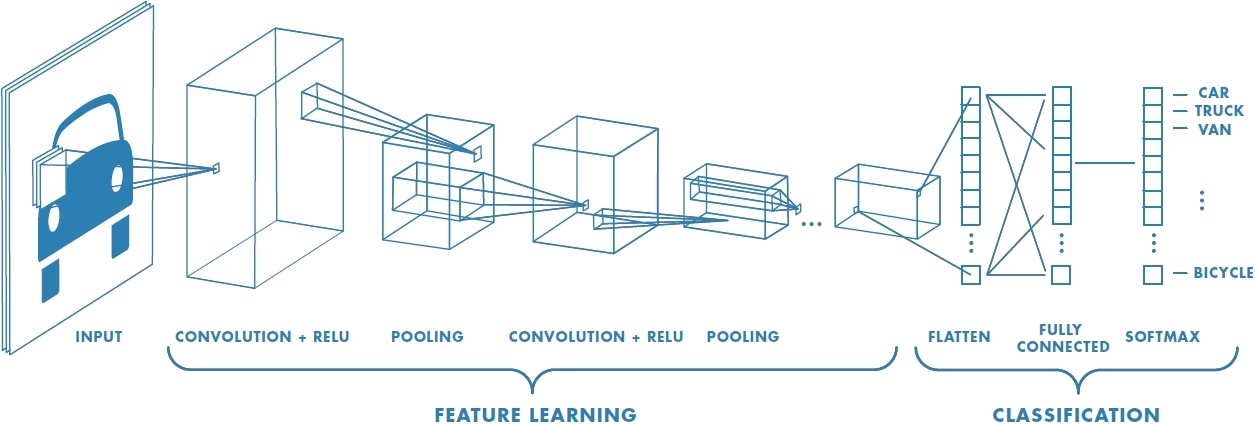
\includegraphics[width=.8\textwidth]{figures/convnet}
\end{center}
\end{frame}

\begin{frame}{Réseaux de neurones et apprentissage profond}
\textbf{Réseaux de neurones récurrents (RNN)}
\begin{itemize}
	\item Utilisé dans les données avec corrélation temporelle et dans le traitement des langues naturelles
	\item Capable de manipuler des entrées de différentes longueurs
\end{itemize}
\begin{center}
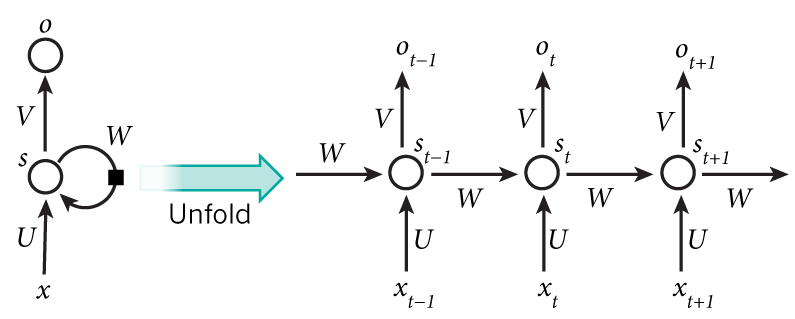
\includegraphics[width=.8\textwidth]{figures/rnn}
\end{center}
\end{frame}

\subsection{Démonstration}

\begin{frame}{Réseaux de neurones et apprentissage profond}

\vspace{0.5cm}
Démonstration : Tensorflow Playground

\begin{figure}[htbp]
\begin{center}
\href{http://playground.tensorflow.org/}{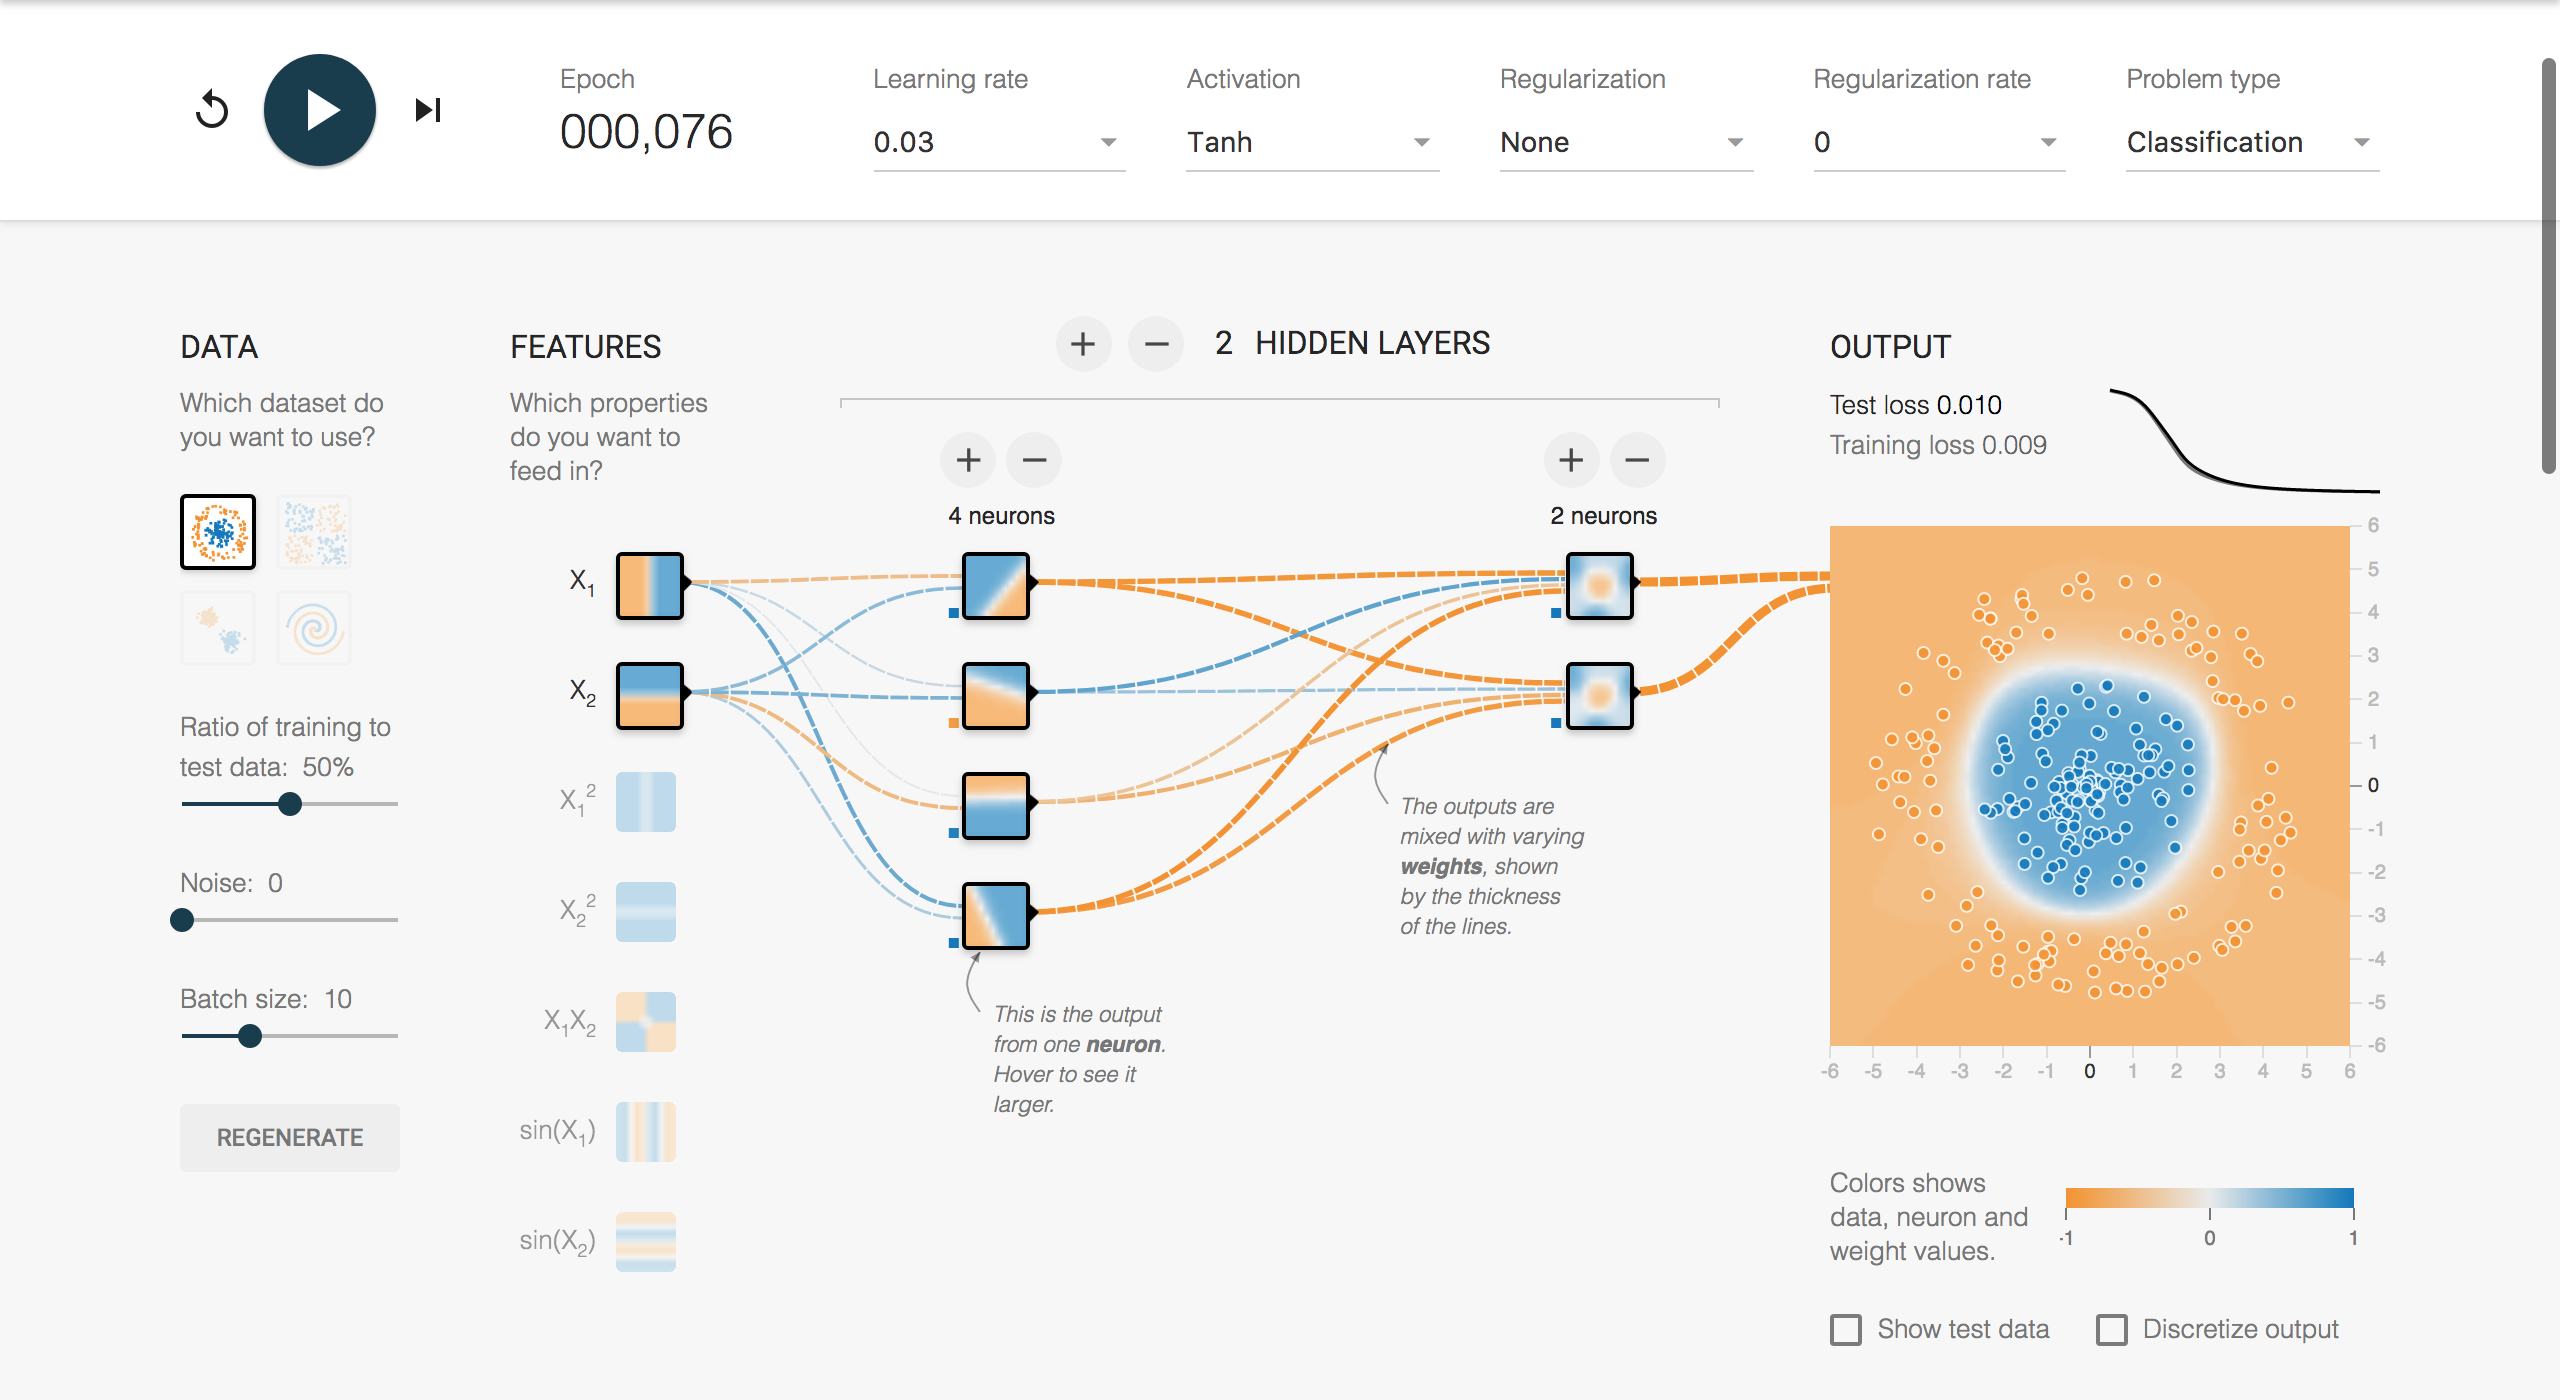
\includegraphics[width=\textwidth]{figures/tensorflow_playground}}
\end{center}
\end{figure}


\end{frame}

\section{Les physiciens dans l'ère du Deep Learning}

\subsection{Beaucoup d'applications...}

\begin{frame}{Les physiciens dans l'ère du Deep Learning}
\begin{center}
{\Large Quelle est la place des physiciens dans tout ça?}
\end{center}
\end{frame}

\begin{frame}{Les physiciens dans l'ère du Deep Learning}
\begin{center}
Beaucoup d'applications possibles dans toutes les branches de la physique!
\end{center}
\textbf{Astronomie}
\vspace{.5cm}
\begin{itemize}
	\item Beaucoup de données $\rightarrow$ potentiel énorme!
	\item exemples:
	\begin{itemize}
		\item Détection d'exoplanètes \cite{2017DPS....4942102P}
		\item Prédiction de phénomènes solaires \cite{McGregor2017}
		\item Détection d'ondes gravitationnelles \cite{George:2017pmj}
	\end{itemize} 
\end{itemize}
\end{frame}

\begin{frame}{Les physiciens dans l'ère du Deep Learning}
\textbf{Matière condensée}
\vspace{.5cm}
\begin{itemize}
	\item Prédiction de l'énergie du niveau fondamental d'un électron \cite{2017arXiv170201361M}
	\item Identification des phases et transitions de phases \cite{carrasquilla2017machine}
\end{itemize}
\vspace{.5cm}
\textbf{Physique des particules}
\vspace{.5cm}
\begin{itemize}
	\item Détection de particules exotiques \cite{2014NatCo...5E4308B}
	\item Caractérisation de jets au LHC \cite{2017arXiv170200748L}
\end{itemize}
\end{frame}

\begin{frame}{Les physiciens dans l'ère du Deep Learning}
\textbf{Climatologie}
\vspace{.5cm}
\begin{itemize}
	\item Détection de phénomènes météorologiques extrêmes \cite{2016arXiv160501156L}
\end{itemize}
\vspace{.5cm}
\textbf{Physique médicale}
\vspace{.5cm}
\begin{itemize}
	\item Détection d'anomalies et de maladies dans une panoplie d'images médicales \cite{2017arXiv170205747L}
\end{itemize}
\vspace{.5cm}
\textbf{Biophysique}
\vspace{.5cm}
\begin{itemize}
	\item Prédiction de repliement de protéines \cite{10.1371/journal.pcbi.1005324}
\end{itemize}
\end{frame}

\subsection{...Et beaucoup de travail en théorie}

\begin{frame}{Les physiciens dans l'ère du Deep Learning}

\begin{center}
Et un grand besoin en théoriciens aussi!
\end{center}
\vspace{.5cm}
\justify
\begin{aquote}{Ali Rahimi\cite{rahimi2017nips}}
"Machine learning has become alchemy - alchemy worked, it helped invented many things. [...] If you are building photo sharing systems, alchemy is OK, but we are beyond that now. We are building systems that govern healthcare and mediate our civic dialogue, we influence elections. I would like to live in a society where systems are built on top of verifiable, rigorous thorough knowledge and not alchemy."
\end{aquote}
\end{frame}

\begin{frame}{Les physiciens dans l'ère du Deep Learning}
\begin{itemize}
	\item \textbf{Pourquoi} est-ce que l'apprentissage profond fonctionne si bien? \cite{2017JSP...168.1223L}
	\item Liens entre l'apprentissage profond et l'intrication quantique \cite{2017arXiv170401552L}
	\item Liens entre l'apprentissage profond et la théorie des champs quantiques ? \cite{2017arXiv171006096F}
\end{itemize}
\end{frame}

\section{Pour aller plus loin...}

\subsection{Librairies Python pour l'apprentissage automatique}

\begin{frame}{Pour aller plus loin...}
\vspace{0.5cm}

Librairies Python pour l'apprentissage automatique

\begin{figure}%
    \centering
    \href{https://www.tensorflow.org/}{\subfloat{{
\includegraphics[height=1.2cm]{figures/logos/tensorflow} }}}%
    \qquad
    \href{http://deeplearning.net/software/theano/}{\subfloat{{
\includegraphics[height=1cm]{figures/logos/theano} }}}%
    \label{fig:example}%
\end{figure}

\begin{figure}
\centering
	\href{http://pytorch.org/}{\subfloat{{
\includegraphics[height=1cm]{figures/logos/pytorch} }}}%
\end{figure}

\begin{figure}%
    \centering
    \href{https://keras.io/}{\subfloat{{
\includegraphics[height=1.2cm]{figures/logos/keras} }}}%
    \qquad
    \href{http://scikit-learn.org/stable/}{\subfloat{{
\includegraphics[height=1.8cm]{figures/logos/scikit_learn} }}}%
    \label{fig:example}%
\end{figure}

\end{frame}

\subsection{Cours et autres ressources}

\begin{frame}{Pour aller plus loin...}

	Cours et autres ressources
	\begin{itemize}
		\item \href{https://admission.umontreal.ca/cours-et-horaires/cours/IFT-3395/}{IFT3395/IFT6390 - Fondements de l'apprentissage machine}
		\item \href{https://www.coursera.org/learn/machine-learning}{Machine Learning sur Coursera}
		\item \href{https://www.youtube.com/user/hugolarochelle}{Chaîne Youtube de Hugo Larochelle}
		\item \href{https://www.youtube.com/channel/UCWN3xxRkmTPmbKwht9FuE5A?&ab_channel=SirajRaval}{Chaîne Youtube de Siraj Raval}
		\item \href{http://karpathy.github.io}{Blog de Andrej Karpathy}	
		\item \href{http://colah.github.io/}{Blog de Chris Olah}		
	\end{itemize}
	
\end{frame}

\section*{Références}

\begin{frame}[t,allowframebreaks]
\setbeamertemplate{bibliography item}{[\theenumiv]}


  \frametitle{Références}
  \nocite*
  \bibliographystyle{siam}
  \bibliography{references}
 \end{frame}

\end{document}